\documentclass[11pt]{article}
\usepackage{graphicx}
\graphicspath{ {images/} }
\usepackage{url}
\usepackage{comment}
\usepackage{epigraph}
\usepackage{float}
\usepackage{wrapfig}
\usepackage{listings}
\usepackage{multirow}
\usepackage{hyperref}
\usepackage{amsfonts}
\usepackage{amsmath}
\usepackage{array}
\usepackage{etoolbox}
\usepackage{yax}
\usepackage{hyperref}
\usepackage{textcomp}
\usepackage[english]{babel} 
\usepackage[nodayofweek]{datetime}

\setparameter Cantrell:
 firstname   = Colin
 lastname    = Cantrell
 title       = {Architect}
 email       = {\href{mailto:colin@nexus.io}{colin@nexus.io}}
 
\setparameter Farinacci:
 firstname   = Dino
 lastname    = Farinacci
 title       = {Protocol Engineer}
 email       = {\href{mailto:farinacci@gmail.com}{farinacci@gmail.com}}
 
\setparameter Smith:
 firstname   = Brian
 lastname    = Smith
 title       = {Core Developer}
 email       = {\href{mailto:brian@nexus.io}{brian@nexus.io}}
 
\setparameter Steve:
 firstname   = Steve
 lastname    = Lackey
 title       = {Core Developer}
 email       = {\href{mailto:steve.lackey@kadima.consulting}{steve.lackey@kadima.consulting}}
 
\setparameter Shea:
 firstname   = Shea
 lastname    = Laver
 title       = {Writer \& Editor}
 email       = {\href{mailto:shea_laver@optusnet.com.au}{shea\textunderscore laver@optusnet.com.au}}
 
\setparameter April:
 firstname   = April
 lastname    = Bunje
 title       = {Writer}
 email       = {\href{mailto:gramalkin75@yahoo.com}{gramalkin75@yahoo.com}}
 
\setparameter Jules:
 firstname   = Jules
 lastname    = Alexandra
 title       = {Writer}
 email       = {\href{mailto:jules@nexus.io}{jules@nexus.io}}
 
\setparameter Nexus:
 firstname   = {Written by some of us,}
 lastname    = {Given as all of us}
 title       = {The Nexus Community}
 email       = {\href{mailto:team@nexus.io}{team@nexus.io}}
 
\newcommand{\printcontributor}[1]{
  \begingroup
  \parindent 0pt
  \usevalue #1: firstname
  \space
  \usevalue #1: lastname
  \ifattribute #1: title {\par}{\relax}
  \usevalue #1: title
  \ifattribute #1: email {\space-\space} {\par\relax}
  \usevalue #1: email
  \endgroup
}

\newcommand{\maketitlepage}[3]{
  \begingroup
  \centering
  
  \vspace*{2\baselineskip}
  
  \textbf{Written by:}\par
  \medskip
  Colin Cantrell\par
  Dino Farinacci\par

  \vspace*{2\baselineskip}

  \textbf{with contributions by:}\par\medskip
  \renewcommand\do[1]{%
    {
    \usevalue ##1:firstname \space \usevalue ##1:lastname \par}%
    }
  \docsvlist{#1}
  \vspace*{2\baselineskip}
  
  \textbf{Edited by:}\par
  \medskip
  Shea Laver
  \\
  \vspace*{3\baselineskip}
  
\includegraphics[width=0.33\textwidth]{./rsz_tritium.png}
  \vspace*{1\baselineskip}
  
\begin{center}
\textit{ad vocem populi}
\end{center}  
  \pagebreak
  \endgroup
}

\newdateformat{usvardate}{%
\monthname[\THEMONTH] \ordinal{DAY}, \THEYEAR}
\newdate{DocDate}{29}{5}{2018}

\begin{document}

\title{\rmfamily\normalfont{Nexus: The Tritium Protocol}}

\date {\usvardate \displaydate {DocDate}}
\maketitle
\begin{abstract}
\begin{center}
\bigskip
\noindent \textit{``Humility is the solid foundation of all virtues"}
\end{center}

\begin{flushright}
Confucius
\end{flushright}
\bigskip

\noindent Blockchain is a flourishing technology that is in a constant state of change.
Nexus is pioneering a new approach to Blockchain technology that solves the biggest challenges faced by the industry, \textbf{\textit{viz.}} scalability, ease of integration, and intuitive user experience.
Beginning with the Tritium update, we are creating an innovative software stack containing multiple layers of abstraction that will streamline business integration into the Nexus framework, form the foundation of a cryptographic identity system, and make smart contracts easily accessible through a feature-rich API set.
Each API call will be developed through a standardization process, with input from businesses, industry leaders and developers, focused on providing a well-designed interface and seamless business integration.

\end{abstract}

\newpage

\tableofcontents
\newpage
\maketitlepage{Shea, Jules, Smith, April, Steve}
\newpage


\paragraph{\textbf{Tritium White Paper} - \textit{1.0.0} - Last Revised \date {\displaydate {DocDate}}  }

\epigraph{nexus: a connection or series of connections linking two or more things.}{\textit{\footnotesize{Oxford English Dictionary}}}
\section{Introduction}

The proposed architecture within this paper combines together a unique set of technologies to increase the processing capabilities of nodes in a distributed system.
By creating a clear distinction between each of these functional components, each layer can be developed and improved independent of one another, processing can be shared across multiple layers, and the integration challenges can be minimized for anyone who chooses to build on this system.


\section{Software Stack}

Following a year of market research, the Nexus software stack follows the principles of modular design, making it uniquely powerful for a range of new use cases. This software stack consists of seven layers, which can be seen below:\\


\hspace{-33pt}
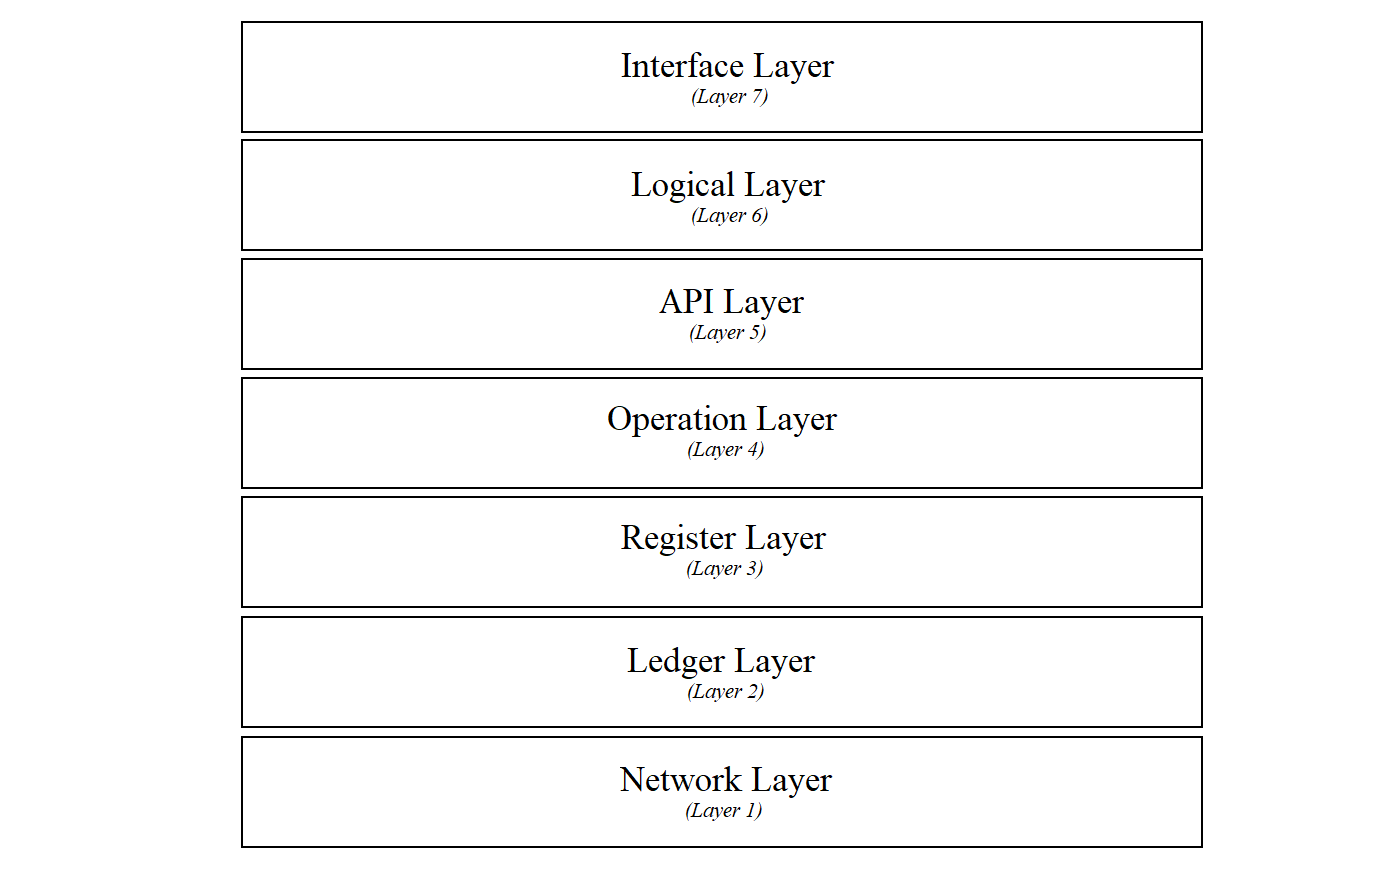
\includegraphics[width=0.9\textwidth]{./images/rsz_stack.png}

\noindent The first layer is considered the Network layer and contains the first six layers of the OSI Reference Model Network Stack.
This is followed by the Ledger layer (3DC) that holds the different data structures representing the distributed database.
The third layer is the Register layer that allows an application to record its state, transfer write permissions to another user, or read the data from a register that acts as a global network-wide address.
The Operation layer is the fourth layer and provides processing capabilities for the Register and Ledger layers.
The standard operation codes and series of codes that act as methods for the object registers will be defined by consensus at annual conferences, ensuring a consistent connection between development and users.
The API layer is the fifth layer of the software stack and will contain a standard set of API calls that executes a series of operations, automating a group of actions that returns the desired result.
The Logical and Interface layers, being the sixth and seventh layers, are the application and user space where most developers and users will interact.
The intuitive design of these layers as distinct functions will provide a premium experience to developers building applications on the Nexus framework.


\section{Network}

\begin{wrapfigure}[10]{r}{0.55\textwidth}
    \centering
    \vspace{-15pt}
    \hspace{0pt}
    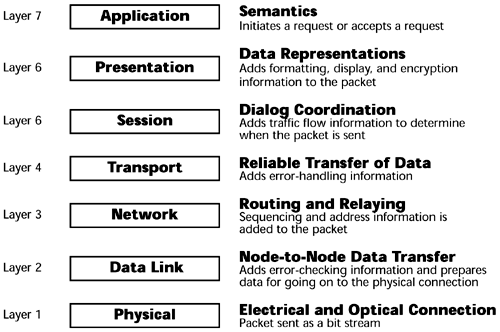
\includegraphics[width=0.55\textwidth]{./images/rsz_osi.png}
\end{wrapfigure}


The Internet is built in layers of software called the ``OSI Reference Model Network Stack'' \cite{NetworkOSI}.
This stack is responsible for all transmission of data from Layer 1 via a physical link to Layer 7, the application space. 
To lay the foundation for viable scaling solutions, certain aspects of the original Blockchain protocol need to be revisited.
Any scaling solution needs to consider how the network propagates messages and which layer it can simplify down to.

\newpage
\subsection{Unicast Flood Networks}

\begin{wrapfigure}[9]{l}{0.50\textwidth}
    \centering
    \vspace{0pt}
    \hspace{0pt}
    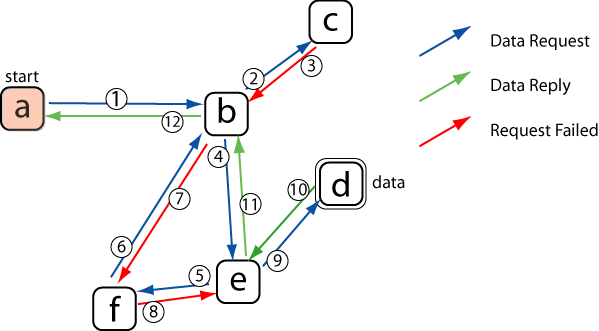
\includegraphics[width=0.50\textwidth]{./images/rsz_flood_network.png}
\end{wrapfigure}

Peer-to-Peer (P2P) networks such as Blockchain require that every message be relayed via unicast \cite{Flood_Networks}, giving rise to the term ``flood network''.
For a message to propagate across the network, all nodes on the network must first process it and then relay it to their peers.
P2P networks gain their robust nature through a large number of active nodes, creating more redundancy in the system.
This redundancy comes at the expense of increased message propagation time and increased ``complexity'' of the routing algorithm, which grows as per $O(n^2)$ \cite{Big_O_Notation}.
This is termed ``exponential time'' and is a highly undesirable complexity for any algorithm other than cryptographic, because as more nodes join the system, they draw exponentially more resources from it.
Thus, cryptocurrency networks must balance the number of nodes required to provide a high degree of redundancy and robustness against the exponential cost of message complexity.

\subsection{Multicast Locking Groups}

\begin{wrapfigure}[9]{r}{0.58\textwidth}
    \centering
    \vspace{-15pt}
    \hspace{0pt}
    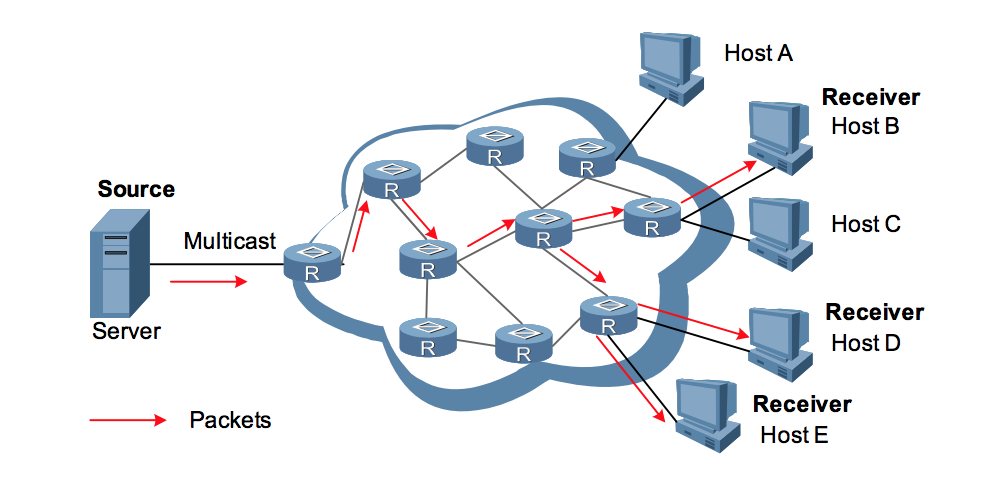
\includegraphics[width=0.58\textwidth]{./images/rsz_multicast.png}
\end{wrapfigure}

Due to the limitations inherent in the basic operation of P2P flood networks, it becomes increasingly clear why distributed ledgers have difficulty scaling.
Scalability is not always determined by the actual size of the ledger, or a state required to be held by all nodes, but also on how the messages route through the network.
Tritium provides an optimized, efficient routing system called ``Multicast Locking Groups'' and is the first step towards Level 1 locking in a multidimensional chaining structure.
As seen in the diagram above \cite{Mulicast}, IP multicast handles the packet replication on the Network layer rather than the Application layer, which significantly speeds up propagation time.
The secondary benefit to running IP multicast in locking groups is that they begin to form parallelism on the Network layer, meaning that messages are broadcast to relevant nodes whilst preserving global consensus layers.
The final benefit is that multicast locking groups can have access control to the groups, which would mean that nodes authorized to broadcast or verify from each of these groups could be easily validated on the ledger.

\subsection{Network Topology}

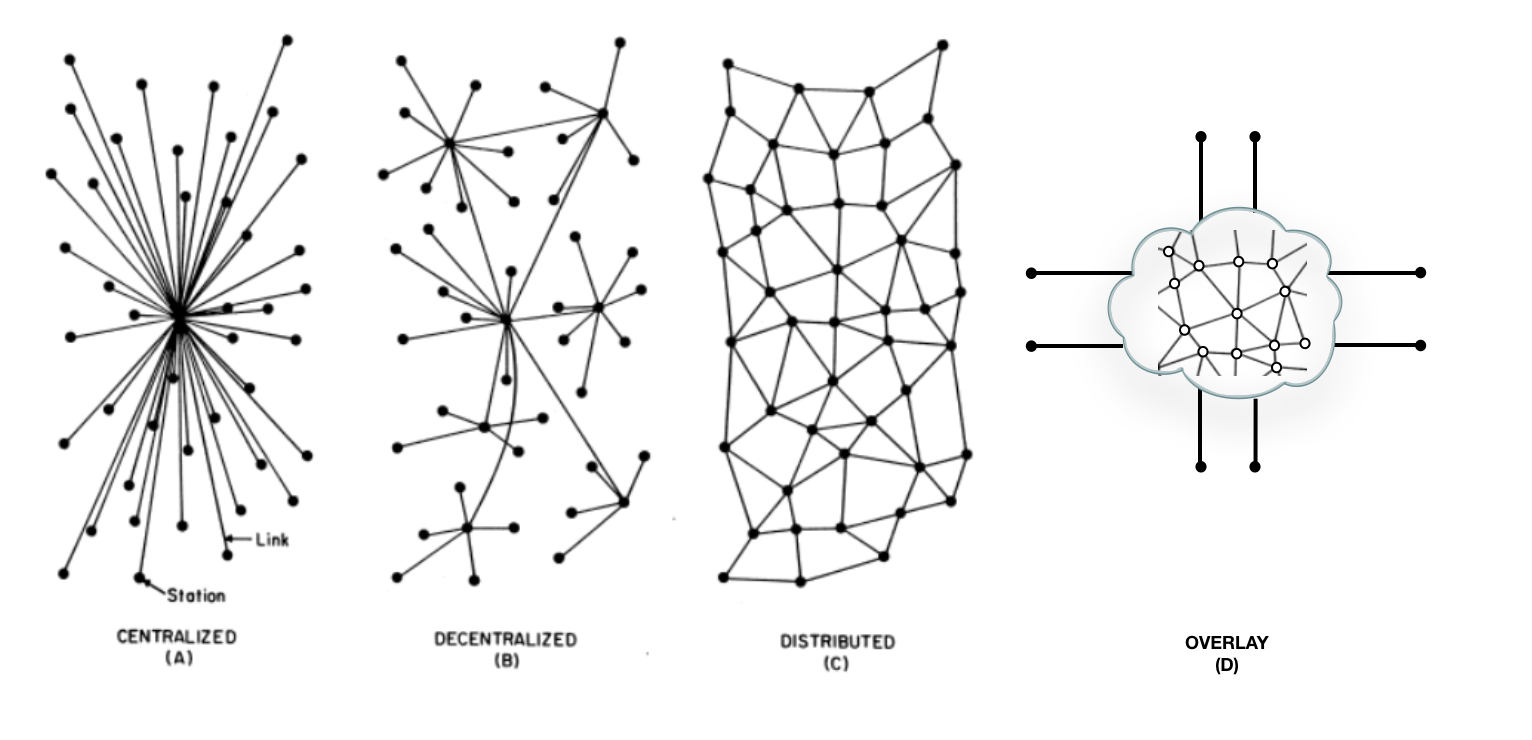
\includegraphics[width=1\textwidth]{./images/rsz_topology.png}

\noindent As seen in the diagram above \cite{Network_Topology}, a distributed topology is an ideal network configuration of great resilience, and while most cryptocurrency networks are assumed to be distributed, consensus mechanisms of other protocols can become decentralized by degrading into several pieces.
This is due to certain limitations of devices that use ``Network Address Translation'' (NAT), which allows devices within a Local Area Network (LAN) to share the same public IP address and route packets to their corresponding device based on port number.
When nodes are behind a NAT, there can be difficulties getting an opening in the NAT for a node to accept incoming connections.
This creates a bottleneck, collapsing a distributed network into a decentralized one.
To solve this, the ~\nameref{sec:LISP}
is included to support an open and secure overlay where Nexus nodes have their own Network layer identity, which maintains a distributed topology regardless of connection method or location.

\newpage
\section{Ledger}

The Ledger layer of the distributed database system is the structure in which transactional data is organized.
Powered by the Lower Level Library, which contains security, database, and protocol messaging services, this layer is the foundation for other applications to be built upon it.
Improvements to the current Blockchain-based ledger are outlined in the following sections.

\subsection{Signature Chains}

\noindent Tritium introduces a new system called ``Signature Chains'' that is designed to increase the security and flexibility of private keys, provide replay protection for account-based transactions, and prevent dust spam attacks.
Signature chains provide username and password functionality which is further protected using a PIN code, removing the need for a wallet.dat file to access your private keys.
This functionality forms the basis for a digital identity system linking every event tied to the signature chain.
The illustration below shows the scheme in more detail.

\medskip
\hspace{-22pt}
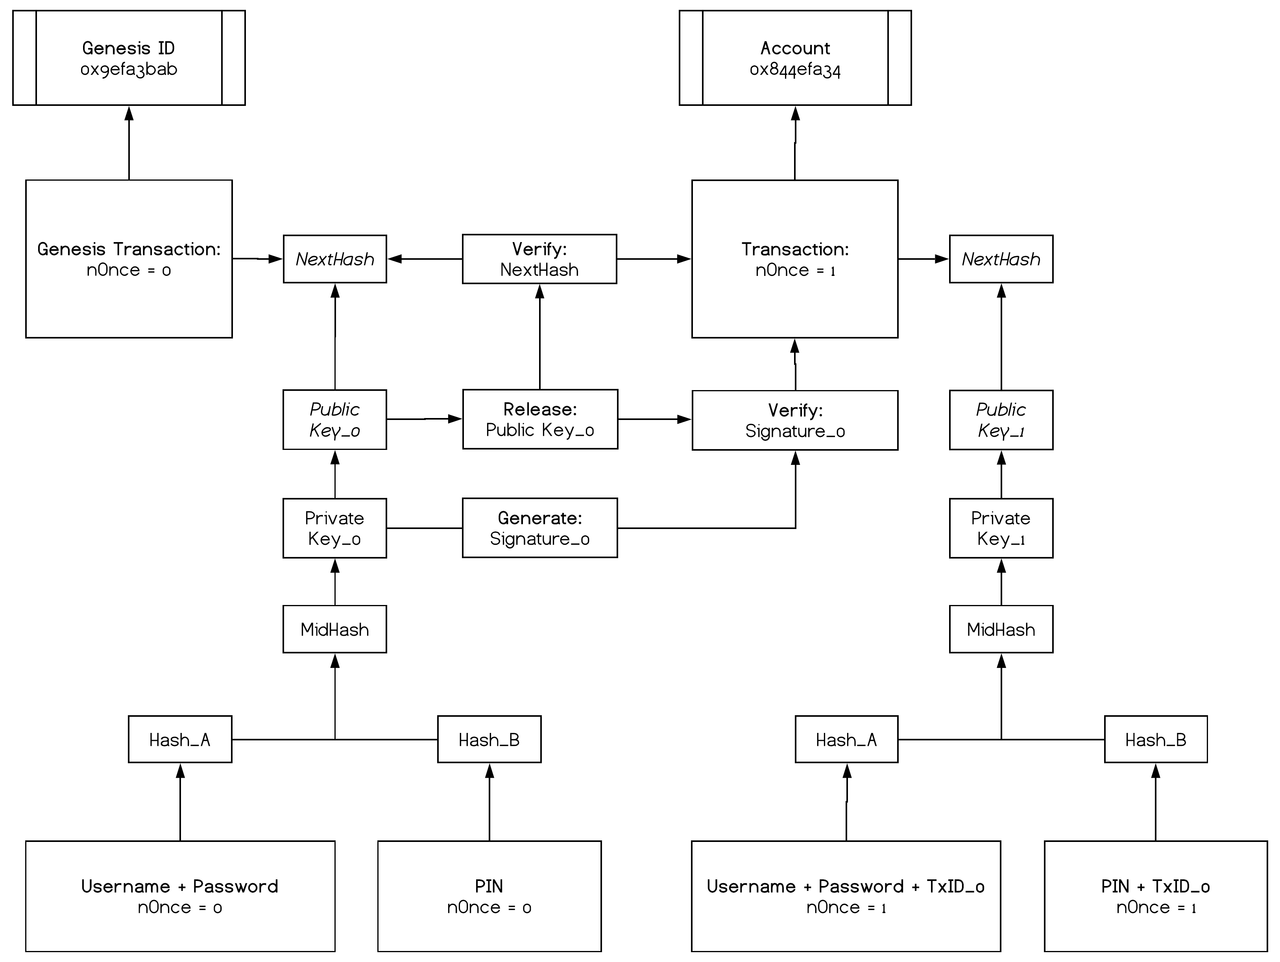
\includegraphics[width=1.00\textwidth]{./images/rsz_sigchains.png}

\subsection{Evolving Signature Scheme}

Signature chains are a quantum-resistant evolving signature scheme developed specifically for Blockchain applications. 
Like the Winternitz signature scheme, it uses a one-time signature (OTS) that signs one message per key. 
The key update algorithm is automatically called after signing a transaction, as a key update is required after every signature.
The key update algorithm takes a secret input provided by the user, a pseudo-random string, and a $n_{ONCE}$ then hashes these inputs multiple times using Skein-Keccak (SK) to form the basis for a private/public key pair based on the Brainpool Standard \cite{Brainpool_Standard}. 
The public key is then hashed using SK-256 to create a 32-byte $NextHash$ that is then published with the transaction data.
This $NextHash$ will be in the form of:

\begin{equation}
\label{eq:NextHash in Chain}
\resizebox{.65\hsize}{!}
{$
N_{h} = Hash_{256}( Hash_{512}( Hash_{1024} ( Pub_{0}, Pub_{1}, ...)))
$}
\end{equation}

\noindent By obscuring keys and sensitive data through hash functions, and by updating the key after every transaction, this signature scheme reduces the window of vulnerability to the period between making a transaction and that transaction being included in the ledger. 
Addresses are no longer tied to the public key of an account and can be reused indefinitely while maintaining maximum security, whereas conventional designs that rely on multiple-use signature schemes become less secure with each use.
The signature scheme outlined above is extremely compact, and it can be adapted to use almost any hash function or asymmetric cryptography.

\subsection{Financial Contracts}

Tritium transactions will no longer contain the UTXO sets as used by Bitcoin and most cryptocurrencies.
Instead, Tritium uses accounts tied as financial contracts to a user's signature chain, which substantially reduces the disk and memory footprint of running a node.
A minimum PoW will be required as a cost when creating an initial account.
Using a signature chain as a decoupled structure from the account prevents the re-use of a key and easily detects conflicting transactions.
This also prevents dust spam attacks and allows transaction fees to be removed.

\subsection{Identity}

Through its qualities of immutability and transparency, a distributed ledger can be considered a trusted platform. Consensus on a series of events or information, i.e. transactions, is publicly verified alongside the attached signature chain, thus it can be referenced to determine whether a certain event has happened or piece of data is accurate.
This forms the basis for an identity system built on the core layers of the technology. By linking accounts to their data and enabling them to verify events on the ledger, users can own their own identity.
Through signature chains, users can access their account on any device through secret information known only to themselves. This sets the stage for more advanced identity markers, as signature chains can be configured to use biometric data such as fingerprints or retinal scans.
Identity is also established at the OSI Network layer through LISP endpoint identifiers (EID).
LISP EIDs are used to give each signature chain a routing identity that maintains integrity across all layers and allows users to make direct P2P connections through their ``cryptographic identity''.
Any attempts to spoof an identity can be prevented as identities can be independently verified on the OSI Network layer and the Ledger layer.
Privacy features can also be implemented by encrypting data packets with LISP on the Network and Presentation layers of the OSI stack.
This provides robust checking and balancing on the Internet by properly linking cryptography with network routes.

\subsection{Reputation}

The mechanism of ``Trust'' is an established mathematical equation based upon the track record of an individual node.
This mechanism functions primarily to build a digital ``reputation'' centered around a series of events that individual nodes have embarked upon, and it will create a reference system for more reputable nodes so that node selection and bias can be more accurate.
Allowing nodes on the network to verify each other through their reputation solves a large issue in most ``Proof-of-Stake'' (PoS) consensus protocols.
By coupling an economic incentive with greater trust, such as higher returns on verification, there is a (non-trivial) cost incurred by loss of reputation.
The key to a good reputation system lies in the effort required in gaining a reputation versus the comparative ease of losing that reputation.
An individual must spend their time and resources supporting the network to build up their reputation in the system.
If an individual were to oppose the collective consensus and pretend certain events have happened, they could have their trust reduced and the viability of their ``witnessing'' decreased.

\subsection{Relationships}

The reputation system is an added layer of protection against attacks that further improves the network's ``Byzantine Fault Tolerance'' \cite{Byzantine}.
While the reputation system can be considered as the public image of each node, the relationship system determines how nodes engage with each other on an individual basis. 
This begins a process of selection bias between nodes, strengthening connections with each other similar to how synapses strengthen in response to activity. 
Under-performing or malicious connections may be pruned and replaced by better, more reliable connections that strengthen the resilience of the network.
This adaptability allows the network to optimize performance, and even measure its performance over time. 
Eventually, nodes can form a private and unique perspective with each other and determine ``normal'' node interactions such as communications, transactions, and other behaviors.
This allows nodes to calculate the validity of another node's ``word'' based on past events in their reputation, coupled with their personal relationships with one another. 
If a node attempts to attack the network, this can be measured against the established ``normal'' series of events and distinguish the attacker.
This lays the foundation of what can be considered an immune system for the global network and consensus mechanism, whereby the network can identify an attack by the departure from normal behavior and neutralize it before sustaining damage.

\subsection{Twin Blocks}

In most current Blockchain technologies, blocks are a single channel data structure which other nodes build upon.
In the case of two blocks being discovered simultaneously, the block accepted by the majority of nodes and built upon is considered as the valid block and is incorporated into the ledger. The other block is abandoned and is known as an \textit{orphaned} block.
When an orphaned block is discovered, the work that successfully produced that block is wasted.
The Tritium Protocol will include \textit{twin blocks} to reduce the possibility of an orphan happening and increase network capacity.
If two blocks of the same height are arranged in the chain of different channels, they will both be accepted as valid if there are no locking conflicts, which is when both blocks contain mutually opposing transactions such as an attempted double spend.
This begins a form of horizontal scaling as well as introducing cross-channel accountability, where multiple block verification channels such as Prime, Hash, or Holding can verify blocks produced by each other.


\section{Register}

\noindent Determining ownership of data in most modern systems depends on third parties in the form of a trusted authority. 
These systems are unable to achieve global consensus or provide immutability and are therefore prone to corruption, theft and other arbitrary weaknesses. 
Distributed ledgers solve these problems and can be further improved through use of a data layer that acts to provide an incontrovertible truth delegated by global consensus.
Understanding this, the Nexus advanced contract engine will be register-based and will act as a state recording machine.
Registers are self-contained objects that hold data associated with the given signature chain that published its most recent state.
This can be more easily understood by the following diagram:

\hspace{-25pt}
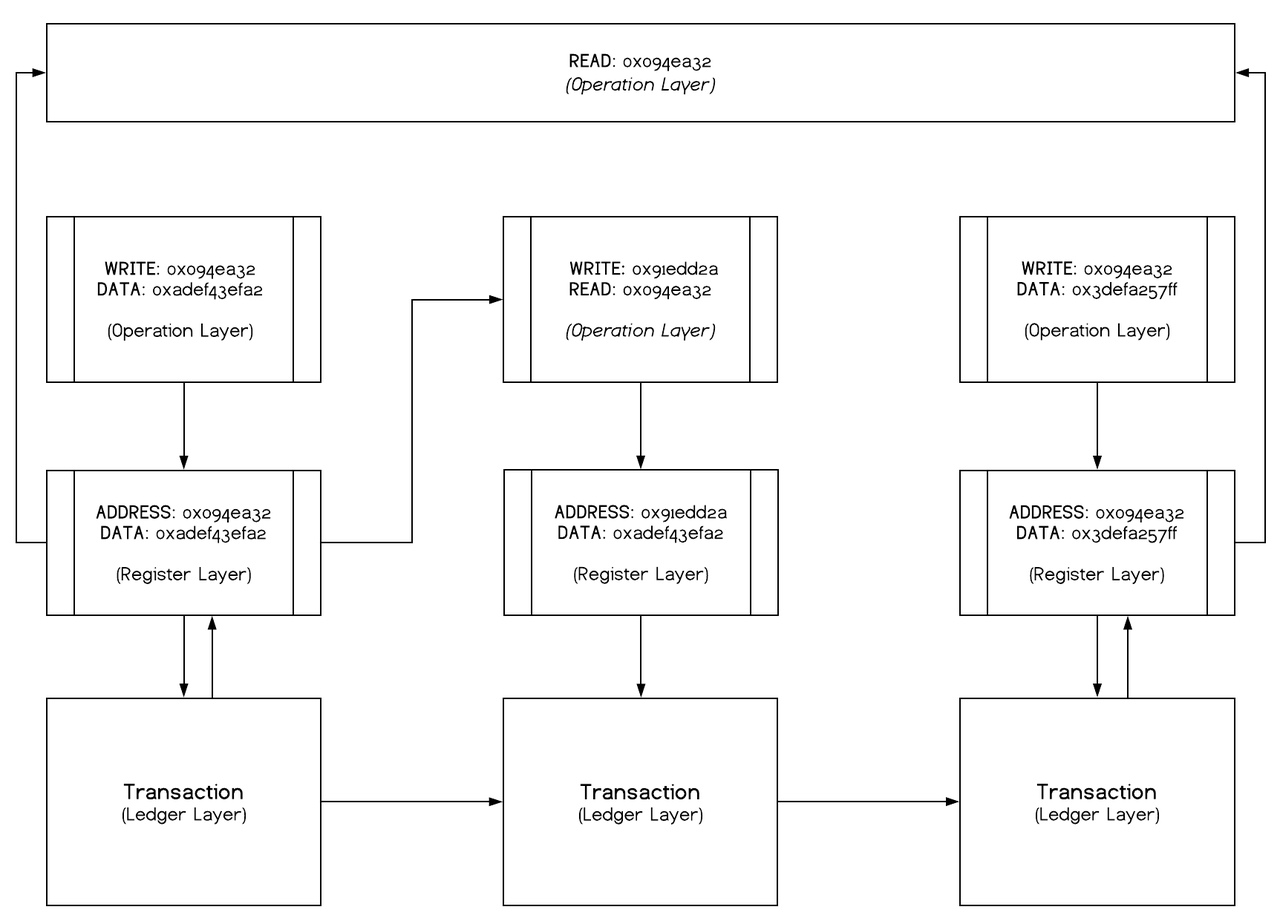
\includegraphics[width=0.95\textwidth]{./images/rsz_registers.png}

\noindent In the diagram above, two transactions record new states through a WRITE operation at register address $0x094ea32$.
The center transaction is performing a WRITE operation to address $0x91edd2a$ with the data from a READ of the most recent state of $0x094ea32$.
Before recording a state, nodes will be required to satisfy all validation scripts for register writes.
The two READ operations above are simple queries to recent states in the register's address and demonstrates different methods of interacting with the Register layer.

\subsection{State Register}

A state register is a register where the ledger deposits raw bytes on a write operation and returns raw bytes on a read operation.
This gives developers the flexibility to serialize data into their registers, updating the state on the ledger while maintaining the interpretation of these byte sequences at the Logical and Interface layers.
This ability means higher levels of abstraction of the ledger can be incorporated without putting unnecessary strain on the processing nodes.
An example of a raw state register could be reference hashes of specific checkpoints in their private databases, to allow the easy verification of data states within internal systems without compromising privacy.
This can be especially useful for systems that require confidentiality, such as medical records or intellectual property.
The Ledger layer will be responsible for ensuring that operations are authorized through an access control scheme and that the register is not placed into an invalid state, such as attempting to write to a read-only register.

\subsection{Object Registers}

Object registers act as their own self-contained objects, similar to how a class functions in object oriented programming.
Object registers can be used for many things including the standardization of specific class formats for meta-data that can be modified by its methods, such as transferring the rights to said meta-data.
Object registers could also reference other object registers as part of a template, enabling the chaining of these data types.
Certain limitations must be placed on the total number of operations and cycles required for each method to ensure that Denial-of-Service (DoS) attacks remain infeasible while providing a unique environment for developers to integrate with distributed ledgers.


\section{Operation}

Operations are byte-level instructions that can be used to perform basic tasks on registers.
The operation codes will require a standardization process and will be thoroughly tested before becoming deployable scripts for the API layer.
These instructions can optionally be compiled from domain specific languages.
These languages can become part of the standards process for generating a series of operations that interact below the API layer and perform tasks desired.


\subsection{Codes}

The following codes can be used to describe some basic functions of the Operation layer:

\begin{enumerate}
\item \textbf{READ}

This operation code will be responsible for returning the contents of a register address by submitting a query to the network that will return that register's most recent state.

\item \textbf{WRITE}

This operation code will be responsible for writing data to a register address. Authors must have the correct authorizations, and the register must not be read-only.

\item \textbf{DEBIT}

This operation will perform a basic subtraction from an available balance in an object register.
This operation will function as a claim ticket to deduct funds from an account when making a transaction, and it will require its counterpart to add those funds to the destination signature chain.

\item \textbf{CREDIT}

This operation will perform a basic addition to an available balance in an object register. It will be the counterpart to the debit transaction sequence and is required to fully move funds from one signature chain to another by proving the series of events leading to the state balance of the sending register.

\item \textbf{TRANSFER}

This operation will transfer the rights to a register of any type, moving the assigned permissions from one signature chain to another.
Data can then be transferred between signature chains or simply show the chain of custody of a specific piece of meta-data, such as a record of ownership of a copyright.

\item \textbf{AUTHORIZE}

This operation will provide an authorization token to a user's register or signature chain, providing proof on the Logical layer that a given public key is valid and authorized to access the services provided.

\item \textbf{GETHASH}

This operation code will be responsible for hashing the data that is submitted as a parameter to it.
For example, this might return the hash of data held at a register address, providing a checksum of the most recent state of said register.

\end{enumerate}

\subsection{Sanitize Inputs}

Object registers can contain methods such as assignment operators for specific data types, which is necessary for the Operation layer to perform the role of sanitizing inputs.
Sanitizing inputs is an important requirement for registers that store specific meta-data formats, which requires each new addition to fit a standard template by the agreed upon process.


\section{API}

Contracts hold the key to the future of distributed systems, although current implementations have issues with accuracy, performance, and ease-of-use. 
These limitations make the implementation process needlessly complicated and expensive, which raises the barriers to entry and leads inevitably to obsolescence.
Considering this, the advanced contract engine will be accessible through an intuitive API set designed specifically for ease-of-use and seamless integration with existing software.
APIs will be accessible through a JSON-REST interface that is globally accessible across the network.
Various APIs will enable developers to push/pull data from the ledger, define terms for new contracts, submit transactions, or define an instance contract for tokenized data.
Rather than using a specific Turing-complete language for access, the front-end can be written in any language preferred by the developer.

\subsection{Gateways}

Node API gateways will provide access to the API layers, with access guided by the gateway's EID. Any node can act as a gateway by advertising their EID as an API gateway.
An API gateway can require authorization by a signature chain message signing key.
Developers on the Logical layer can implement calls through these gateways to interact with the lower levels of the software stack.

\subsection{API Types}

There are many different industries that will require industry-specific APIs, including medical, copyright, finance, and identity.
Each API will function according to the standards set by the standardization process, executing a series of operations through the Operation layer that will interact with registers and validate states through the ledger.

\subsection{Standards}

The APIs, along with the processes on the Operational layer, will be decided through a standards process at regular conferences.
The model will be similar to the Internet Engineering Task Force (IETF) standards such as Request for Comments (RFC) and Internal Standard Organization (ISO), and will allow businesses to help define new operational methods for object registers, along with new API calls for industry-specific API sets.
Consultation is considered necessary for the successful adoption of distributed ledger technology, ensuring that development continues to meet user needs and that the ledger can evolve to the exacting new standards.


\section{Logical}

The Logical layer is the core application space of the software stack.
Applications built on the Nexus framework will use the API layer to interact with the network, apply new states to registers, execute register operation methods, or authorize to signature chains. Some examples ~\nameref{sec:Applications} can be found in the appendix.

\subsection{State Recording}

The Logical layer could, through its abstraction layer, use the ledger as a state recording machine to record new states of its program.
These would be key checkpoints to the main system, using the immutable ledger as a reference point for recent states in distributed applications.
Arbitrary data can be interpreted from the Logical layer by de-serializing any input data in and out of a state register.

\subsection{Data Chaining}

Data chaining enables full control of one's own data in a manner that others can reference and utilize through the Logical layer. This allows the creation of various checks and balances, as verification of that data can be performed by one's peers.
Signature chains are a core component of data chaining as each chain is established with their own record of events according to what they publish.

\subsection{Authorization}

Signature chains can form the basis for an access control scheme, by restricting or granting access to specific data such as contracts or multi-signature accounts.
In the API functions, standard authorization calls can be used to publish an access list containing specified public keys that authorizes access to data on a private network.
This will also provide the Logical layer the opportunity for encrypting data with this published and authorized public key, and also be a record keeper of the signature chains that have requested access to certain components of the Logical layer.


\section{Interface}

The Interface layer will improve the accessibility of the Ledger layer by interacting through API calls and operation codes.
Through two major areas of focus \textit{\textbf{viz.}} a decoupled daemon and modular design, interface design becomes simpler yet more powerful
.
Developers can focus on providing an intuitive and responsive UI instead of the intricacies of Blockchain design.

\subsection{Decoupled Daemon}

As currently implemented, the qt-wallet couples the graphical user interface (GUI) with the actual daemon-level operations, which creates an unresponsive, poor user experience.
The Nexus user interface (UI) will be a stand-alone application running independently of the daemon, which will run in the background. This allows for seamless updates to the core software, and automatic reloading and bootstrapping to occur in the background with minimal user interruption.

\subsection{Modular Design}

Modular design is an important aspect of system architecture, providing a more robust and stable software platform as modules run on individual processes separate from the main application. 
Modules can then be developed to meet future needs or perform specific tasks and provides greater flexibility and extensibility.
The user interface adopts this approach and grants the end-user full control over their UI, allowing them to select and install modules as needed.
This allows developers to create an array of new use cases limited only by imagination, creativity, and available technology.
This will engender the birth of a marketplace where developers can share and sell custom modules built for the Nexus interface.


\section{Security Considerations}

\noindent This section delves deeper into the mathematical foundations underpinning signature chains as a signature scheme. 
It explores the relative quantum resistance for signature chains through the combination of Grover's algorithm and Shor's algorithm. 
This section uses Big O notation \cite{Big_O_Notation} to depict the number of iterations required to successfully attack a given encryption.\\

\subsection{Attacking the NextHash in SigChains}

\noindent As explained earlier in this document, we can determine how a $NextHash$ ($N_{h}$) is generated: 

\begin{equation}
\label{eq:Next Hash in Chain}
\resizebox{.55\hsize}{!}
{$
N_{h} = Hash_{256}( Hash_{512} ( Hash_{1024}(Pub_{n}))) 
$}
\end{equation}
\\
\noindent This can be reversed into the public key by Grover's algorithm requiring:

\begin{equation}
\label{eq:Iterations required to reverse the public key from a NextHash}
\resizebox{.35\hsize}{!}
{$
= O(2^{128} + 2^{256} + 2^{512})
$}
\end{equation}
\\
\noindent Retrieving the private key from a reversed $NextHash$ in a signature chain would require an additional $O(512^3)$ iterations. Therefore, one would have the very last private key in that signature chain with a total of:

\begin{equation}
\label{eq:Total Iterations to Reverse Private Key from $N_{h}$ }
\resizebox{.45\hsize}{!}
{$
= O(2^{128} + 2^{256} + 2^{512} + 512^{3})
$}
\end{equation}

\noindent Access to this private key allows one to claim ownership of the signature chain and the associated balance of NXS or data.
The number of iterations illustrated above is an astronomical number and is above the recommended cryptographic standard for Top Secret \cite{Topsecret_Standard}.
This makes it suitable for the emerging quantum age.\\

\subsection{Attacking vulnerable public keys}

\noindent Another security consideration concerns the ability of quantum computers to attack vulnerable public keys.
Signature chains keep the active keys obscured until a transaction is made and only the public key is ever published.
This protects active keys against Shor's algorithm, but once the public key is published then quantum computers with approximately 3500-qubits could attack the public key over running time $O(n^3)$.
If a quantum computer were able to break an old public key and reveal the corresponding private key, it would be in a position to attack the master base hashes.
This is the process of generating the $MidHash$:

\begin{equation}
\label{eq:}
\resizebox{.70\hsize}{!}
{$
= Hash_{512}(Hash_{1024}(Secret_{A}) + Hash_{1024}(Secret_{B}))
$}
\end{equation}

\noindent To further increase entropy, each secret input is combined with a pseudorandom string generated from the previous transaction. Thus, the creation of a signature chain is the result of hashing data points known to the user but unknown to the attacker.

\begin{equation}
\label{eq:Iterations required to discover seeds}
\resizebox{.35\hsize}{!}
{$
 = O(2^{256} + 2^{512} + 2^{512})
$}
\end{equation}

\noindent This shows how the master secret phrases ($Secret_{A}$ and $Secret_{B}$) can be secured at above a 512-bit quantum standard.\\

\subsection{Brute Forcing Weak Secret Seeds}

Another attack that could be used is known as a dictionary attack, where a key pair is generated by brute forcing inputs from a word list.
The generated public key would then be hashed and compared against the $NextHash$ to see if it unlocks a user's signature chain.
If someone were to use a weak username, password, or PIN, the ability to attack it with dictionary attacks would be greatly increased by the weakness of the password. 

\begin{equation}
\label{eq: Iterations to Dictionary Attack}
\resizebox{.17\hsize}{!}
{$
O(\frac{2^{128} \cdot 2^{16}}{k})
$}
\end{equation}

\noindent In the figure above, variable $k$ demonstrates the relationship between the complexity of your password versus the complexity of the dictionary attack with a $Secret_{A}$ minimum entropy of 128 bits, and a $Secret_{B}$ minimum entropy of 16 bits.
The larger the word list used by the attack, the greater the chances of successfully brute-forcing the seed data that generates the $MidHash$.
The greater the entropy in $Secret_{A}$ and $Secret_{B}$, the less chance there is that an attacker will successfully find the $MidHash$.


\section{Conclusion}

The Tritium Protocol as described in this document is the first of three updates named Tritium, Amine and Obsidian (TAO).
Inspired by the principles of modular design, these updates represent a new stage of Blockchain development that addresses the critical issues facing existing technology. 
They bring remarkable improvements in efficiency, scalability, and security through the intelligent use of the cryptography, architecture, and software layers that power Nexus.
The \textit{\textbf{magnum opus}} of the Tritium upgrade is the register-based smart contract engine.
This engine provides the opportunity to directly own, transfer, lease, or publish data that can be securely utilized, distributed and/or monetized.
It is the first step towards a practical and efficient distributed system that can be tailored to various use cases. Through an intuitive user interface and comprehensive API sets, Tritium enables seamless integration with other applications.
With the upcoming release of key elements of Tritium, there is plenty to be excited about.

\pagebreak

\appendix

\section{Appendix: More content for those inclined}

If you seek more details about the Tritium protocol or content to reinforce what has been written above, please continue reading.

\epigraph{The real danger is not that computers will begin to think like men, but that men will begin to think like computers. - Sydney Harris}


\section{Update Phases}

The fundamental Contract phases are outlined through the three stages of the TAO framework.
With each update, new components of the contracting engine will be released.
This reduces overall contract complexity by isolating the simplest and most useful features, and allows businesses that are building on the Nexus software stack to have input on the forward development and outlines of the standards for each release.
This is very important for streamlining the integration between consumers, businesses, and networks, as every component complements one another such that none can exist in isolation.

\section{Applications}
\label{sec:Applications}

The following sections will outline some of the practical use cases in a post-Tritium development environment.
These use cases build upon different aspects of the network ledger such as reputation, contracts, and register states.

\subsection{Receive Accounts}

The incorporation of advanced contracts into the software stack allows the generation of receive accounts with built-in smart financial instruments, such as stipulations on funds received and their appropriation.
Such instruments could prevent a holder from receiving funds deposited into their account from an unapproved source or origin, require a receive signature from the receive account i.e. a receipt, or prevent funds from being sent to an invalid address.
Extrapolating further, smart financial instruments such as receive signatures can be expanded into a form of multi-signature contracts, where senders of funds into the receive address would be required to sign together for the movement of any of the funds.
In the case of crowd funding or decentralized autonomous organizations, contributors or members are able to decide together how the funds are spent, increasing accountability and transparency.

\subsection{Ledger Level DAO}

A Decentralized Autonomous Organization's (DAO) guiding principle is the foundation of an organization-wide democratic process governing all funding proposals.
In an industry rife with speculation and ``Initial Coin Offerings'' (ICOs) attracting millions in funding, a DAO provides both accountability and transparency.
In the following example, we propose a DAO structure that can be built on the Nexus framework.
First, this DAO would receive an organizational signature chain, with other ``founders'' of the organization as the other signatories.
The data chain can publish certain references to by-laws or simply rest on the genesis transaction.
When making a funding proposal, they would create a receive account contract with stipulations and a requirement for the movement of any NXS be collected by a token vote.
This collective authorization can be seen by the diagram below:

\hspace{-25pt}
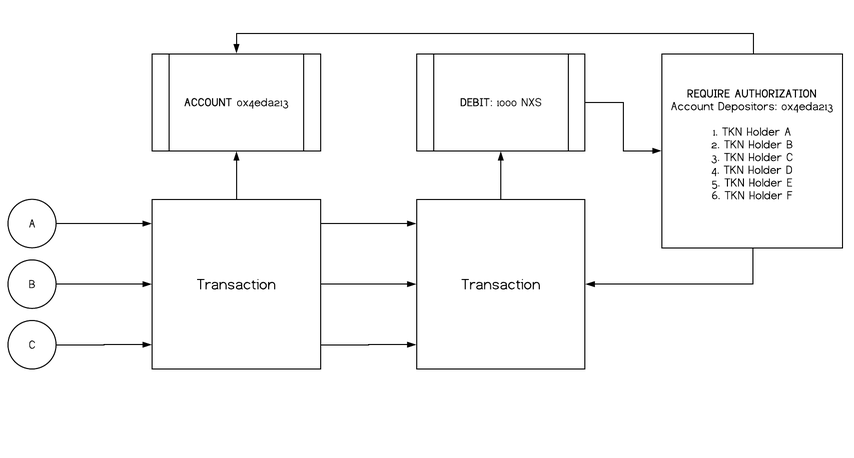
\includegraphics[width=1.00\textwidth]{./images/rsz_dao.png}
\pagebreak

\noindent Token issuer(s) \textit{(A, B, and C in the above diagram)} would be required to propose a budget at the initial fund raising event, and for their token holders to ratify future movements of tokens.
This creates a secure ledger-level series of organizational contracts that allows businesses, consumers, and investors to function in a more streamlined and connected way.
Nexus aims to transition the Nexus Embassy(s) into a global DAO called a Distributed Autonomous Community (DAC) and in so doing, honor its founding principles: by the people, for the people.
More details on how this will function will be delivered in the Obsidian white paper.

\subsection{Tokenized Data}

Signature chains can prove ownership on a distributed ledger by publishing a meta-data representation (token data) regarding a work of art, a logo or slogan, a domain name allocation, patents or copyrighted material.
Anyone can access copyrighted material by simply purchasing and holding the token from a secondary market.
As requirements for this data are set within the parameters of the copyright contract, when someone pays a license fee for the use of this published data, this fee is then distributed to the token holders.
This concept will enable anyone to buy or sell shares representing physical objects, art, music or any other agreed means, allowing anyone to create, distribute and monetize on a single, accessible platform.

\subsection{Supply Chains}

Signature chains and cryptographic identity can also facilitate supply chains, which are often cumbersome and inefficient.
Supply chains on a distributed ledger can trace the history of products from start to finish, providing trustworthy information regarding standards and certifications.
Advanced contracts can automate many processes, eliminating costly delays and reducing double handling.
Greater transparency of supply chains can allow consumers to make informed choices that reward sustainable and ethical practices.

\newpage
\section{Locator/ID Separation Protocol (LISP)}
\label{sec:LISP}

\subsection{Level of Indirection for Addressing and Routing}

LISP operates at the OSI Network layer and is an architecture that decouples an address identity from address location. In the current Internet architecture, an IP address combines who you are with where you are connected to the network. 
LISP extends the Internet architecture in an incremental and compatible way to allow IP addresses to come in two forms, end-point IDs (EIDs) and routing locators (RLOCs). 
This level of indirection allows network overlays to be built where EIDs are on the periphery of the overlay, and RLOCs are routable addresses in the Internet underlay routing system that operates today.
The performance of the underlay routing system remains unchanged, as the mapping and linking of EIDs to RLOCs occurs entirely on the overlay.

\subsection{Nexus over LISP}

\noindent The Nexus applications and daemons, which run at the OSI Application layer, send unicast and multicast packets that are sent and received by EID addresses. LISP, which runs at the OSI Network layer, finds where EIDs are topologically located by looking up EID addresses in a mapping system. 
The mapping system is decentralized and distributed for security and scalability and is used to find one or more RLOCs for an EID.\\

\noindent Each Nexus wallet or miner is assigned a single EID address. 
If the Nexus node has multiple network interfaces, they are assigned either statically or dynamically with an RLOC address. 
LISP registers a signed mapping for EID-to-RLOCs to the mapping system. 
If the Nexus node moves, the EID remains allocated and new RLOCs are allocated and registered by LISP to the mapping system.
This allows applications to remain connected without needing to deal with node mobility issues.\\

\noindent Nexus nodes can also be grouped in LISP multicast groups, which can be addressed through IP multicast group addresses. The LISP mapping system tracks and authenticates the location of nodes on the overlay, even as they change physical location or connection point.

\subsection{Another Layer of Security}


\noindent The LISP overlay provides another layer of security for Nexus applications by supporting crypto-EIDs, which are similar to Nexus wallet addresses. 
Crypto-EIDs are hashes of public-keys where the mapping system stores public-keys and performs LISP message verification on each control-plane message. 
At the data-plane, all Nexus packets sent on the overlay are encrypted and contain packet integrity checking so packets are immutable and cannot be eavesdropped on.\\

\noindent The LISP overlay makes use of several state of the art cryptographic mechanisms.
In the control-plane, ECDSA and SHA-256 are used for digital signatures with dynamic one-time key exchange. 
In the data-plane, many cipher-suites are available for packet encryption and integrity verification such as AES-CBC, AES-GCM, ChaCha20 ciphers, and SHA256 and Poly1305 ICV hash functions using Elliptic-Curve 25519 dynamic key exchange.

\noindent For the Nexus user, this level of security allows your communications to remain private, preventing any eavesdropping between peers.

\subsection{Advanced Level of Scalability}

\noindent Since many computers and devices sold today have multiple network interfaces, they are usually only used to provide redundancy.
So if the Wi-fi interface goes down then the LTE interface is used.
When Nexus and LISP run together on a device, each network interface is assigned an RLOC address. 
Remote nodes that want to communicate can use either a RLOC address or load-share traffic across all your network interfaces.
The remote node can even test for "underlay distance and latency" and switch back and forth, or disproportionately send to one RLOC versus another.\\

\noindent The integration of Nexus and the LISP overlay helps achieve scalability through reduced network latency in a truly unique manner. Furthermore, the 32-bit IPv4 address used by most network protocols will be unable to support the future growth of networked devices. Nexus and the LISP overlay will use 128-bit IPv6 EID addresses that can accommodate far more devices on the network.\\

\noindent Together, Nexus and LISP form the world's first truly distributed, secure and scalable application and infrastructure network.

\subsection{Open Standards and Open Source}

\noindent LISP began in the Internet Research Task Force (IRTF) in 2007 and then transitioned to standards development in the Internet Engineering Task Force (IETF) in 2009. 
Use case development and protocol extension work still continues in the IETF LISP Working Group which meets 3 times a year. 
There are many vendor and open-source implementations available and thousands of deployments in enterprise and service provider environments.\\

\noindent For more information about LISP, you can find presentations, demos, testimonials, and detail specifications at http://www.lispers.net. 

\newpage

\section{List of Contributors}

\begingroup
\parindent 0pt
\parskip  8pt

\begin{enumerate}
\item 
\printcontributor{Cantrell}

\item
\printcontributor{Farinacci}

\item
\printcontributor{Shea}

\item
\printcontributor{Jules}

\item
\printcontributor{Smith}

\item
\printcontributor{April}

\item
\printcontributor{Steve}

\item
\printcontributor{Nexus}
\end{enumerate}

\endgroup


\pagebreak
\begin{thebibliography}{7}


%\bibitem{NetworkOSI}
%OSI Reference Model Network Stack Diagram
%\url{http://nadav.media.mit.edu/index.html%3Fn=Projects.SocialAreaNetworks.html}

\bibitem{NetworkOSI}
The OSI Reference Model and Protocols
\url{https://flylib.com/books/en/2.567.1.38/1/}

\bibitem{Flood_Networks}
Unicast Flood Networks
\url{https://www.studeersnel.nl/nl/document/avans-hogeschool/informatiebeveiliging/werkstukessay/paper-deep-en-dark-web/1320073/view}

\bibitem{Multicast}
Classification of Multicast Routing Protocols
\url{https://www.researchgate.net/figure/Classification-of-Multicast-Routing-Protocols_fig2_278023165}

\bibitem{Big_O_Notation}
Big O Notation
\url{https://www.khanacademy.org/computing/computer-science/algorithms/asymptotic-notation/a/big-o-notation}

\bibitem{Byzantine}
Guru: Universal Reputation Module for Distributed Consensus Protocols
\url{https://eprint.iacr.org/2017/671.pdf}

\bibitem{Network_Topology}
Network Routing Topology
\url{https://retroshare.readthedocs.io/en/latest/concept/topology/}

\bibitem{Brainpool_Standard}
Elliptic Curve Cryptography (ECC) Brainpool Standard Curves and Curve Generation
\url{https://tools.ietf.org/html/rfc5639}

\bibitem{Topsecret_Standard}
Cryptographic Key Length Recommendation from organizations
\url{https://www.gronau-it-cloud-computing.de/en/cryptographic-key-length-recommendation-from-organizations/}

\end{thebibliography}

\end{document}
